\documentclass[12pt,a4paper]{article}
\usepackage{lmodern}

\usepackage{placeins}
\usepackage{amssymb,amsmath}
\usepackage{ifxetex,ifluatex}
\usepackage{fixltx2e} % provides \textsubscript
\ifnum 0\ifxetex 1\fi\ifluatex 1\fi=0 % if pdftex
  \usepackage[T1]{fontenc}
  \usepackage[utf8]{inputenc}
\else % if luatex or xelatex
  \ifxetex
    \usepackage{mathspec}
    \usepackage{xltxtra,xunicode}
  \else
    \usepackage{fontspec}
  \fi
  \defaultfontfeatures{Mapping=tex-text,Scale=MatchLowercase}
  \newcommand{\euro}{€}
\fi
% use upquote if available, for straight quotes in verbatim environments
\IfFileExists{upquote.sty}{\usepackage{upquote}}{}
% use microtype if available
\IfFileExists{microtype.sty}{%
\usepackage{microtype}
\UseMicrotypeSet[protrusion]{basicmath} % disable protrusion for tt fonts
}{}
\usepackage[lmargin = 5cm,rmargin = 2.5cm,tmargin = 2.5cm,bmargin =
2.5cm]{geometry}

% Figure Placement:
\usepackage{float}
\let\origfigure\figure
\let\endorigfigure\endfigure
\renewenvironment{figure}[1][2] {
    \expandafter\origfigure\expandafter[H]
} {
    \endorigfigure
}

%%%% Jens %%%%
\DeclareMathOperator*{\argmax}{arg\,max}
\DeclareMathOperator*{\argmin}{arg\,min}
\DeclareMathOperator{\bc}{bc}
\DeclareMathOperator{\poly}{poly}

%%%% table %%%%
\usepackage{lscape}
\renewcommand{\arraystretch}{1.5}

\usepackage{numprint}
\npthousandsep{\,}

%% citation setup
\usepackage{csquotes}

\usepackage[backend=biber, maxbibnames = 99, style = apa]{biblatex}
\setlength\bibitemsep{1.5\itemsep}
\addbibresource{R_packages.bib}
\bibliography{references.bib}
\usepackage{graphicx}
\makeatletter
\def\maxwidth{\ifdim\Gin@nat@width>\linewidth\linewidth\else\Gin@nat@width\fi}
\def\maxheight{\ifdim\Gin@nat@height>\textheight\textheight\else\Gin@nat@height\fi}
\makeatother
% Scale images if necessary, so that they will not overflow the page
% margins by default, and it is still possible to overwrite the defaults
% using explicit options in \includegraphics[width, height, ...]{}
\setkeys{Gin}{width=\maxwidth,height=\maxheight,keepaspectratio}
\ifxetex
  \usepackage[setpagesize=false, % page size defined by xetex
              unicode=false, % unicode breaks when used with xetex
              xetex]{hyperref}
\else
  \usepackage[unicode=true, linktocpage = TRUE]{hyperref}
\fi
\hypersetup{breaklinks=true,
            bookmarks=true,
            pdfauthor={Jens Klenke and Janine Langerbein},
            pdftitle={P-Approximation},
            colorlinks=true,
            citecolor=black,
            urlcolor=black,
            linkcolor=black,
            pdfborder={0 0 0}}
\urlstyle{same}  % don't use monospace font for urls
\setlength{\parindent}{0pt}
\setlength{\parskip}{6pt plus 2pt minus 1pt}
\setlength{\emergencystretch}{3em}  % prevent overfull lines
\setcounter{secnumdepth}{5}

%%% Use protect on footnotes to avoid problems with footnotes in titles
\let\rmarkdownfootnote\footnote%
\def\footnote{\protect\rmarkdownfootnote}

%%% Change title format to be more compact
\usepackage{titling}

% Create subtitle command for use in maketitle
\newcommand{\subtitle}[1]{
  \posttitle{
    \begin{center}\large#1\end{center}
    }
}

\setlength{\droptitle}{-2em}
  \title{P-Approximation}
  \pretitle{\vspace{\droptitle}\centering\huge}
  \posttitle{\par}
\subtitle{Seminar in Econometrics}
  \author{Jens Klenke and Janine Langerbein}
  \preauthor{\centering\large\emph}
  \postauthor{\par}
  \predate{\centering\large\emph}
  \postdate{\par}
  \date{today}

\usepackage{booktabs}
\usepackage{longtable}
\usepackage{array}
\usepackage{multirow}
\usepackage{wrapfig}
\usepackage{float}
\usepackage{colortbl}
\usepackage{pdflscape}
\usepackage{tabu}
\usepackage{threeparttable}
\usepackage{threeparttablex}
\usepackage[normalem]{ulem}
\usepackage{makecell}
\usepackage{xcolor}

%% linespread settings

\usepackage{setspace}

\onehalfspacing

% Language Setup

\usepackage{ifthen}
\usepackage{iflang}
\usepackage[super]{nth}
\usepackage[ngerman, english]{babel}

%Acronyms
\usepackage[printonlyused, withpage, nohyperlinks]{acronym}
\usepackage{changepage}

% Multicols for the Title page
\usepackage{multicol}

\begin{document}

\selectlanguage{english}

%%%%%%%%%%%%%% Jens %%%%%
\numberwithin{equation}{section}


%\maketitle

\begin{titlepage}
  \noindent\begin{minipage}{0.6\textwidth}
	  \IfLanguageName{english}{University of Duisburg-Essen}{Universität Duisburg-Essen}\\
	  \IfLanguageName{english}{Faculty of Business Administration and Economics}{Fakultät für Wirtschaftswissensschaften}\\
	  \IfLanguageName{english}{Chair of Econometrics}{Lehrstuhl für Ökonometrie}\\
  \end{minipage}
	\begin{minipage}{0.4\textwidth}
	  \begin{flushright}
  	  \vspace{-0.5cm}
      \IfLanguageName{english}{\includegraphics*[width=5cm]{Includes/duelogo_en.png}}{\includegraphics*[width=5cm]{Includes/duelogo_de.png}}
	  \end{flushright}
	\end{minipage}
  \\
  \vspace{0.25cm}
  \begin{center}
  \huge{P-Approximation}\\
  \vspace{.25cm}
  \Large{Seminar in Econometrics}\\
  \vspace{0.5cm}
  \large{Term Paper}\\
  \vspace{0.5cm}
  \large{  \IfLanguageName{english}{Submitted to the Faculty of \\  Business Administration and Economics  \\at the \\University of Duisburg-Essen}{Vorgelegt der \\Fakultät für Wirtschaftswissenschaften der \\ Universität Duisburg-Essen}\\}
  \vspace{0.75cm}
  \large{\IfLanguageName{english}{from:}{von:}}\\
  \vspace{0.5cm}
  Jens Klenke and Janine Langerbein\\
  \end{center}
  %\vspace{2cm}
  \vfill
  \hrulefill

  \noindent\begin{minipage}[t]{0.3\textwidth}
  \IfLanguageName{english}{Reviewer:}{Erstgutachter:}
  \end{minipage}
  \begin{minipage}[t]{0.7\textwidth}
  \hspace{1cm}Christoph Hanck
  \end{minipage}

  \noindent\begin{minipage}[t]{0.3\textwidth}
  \IfLanguageName{english}{Deadline:}{Abgabefrist:}
  \end{minipage}
  \begin{minipage}[t]{0.7\textwidth}
  \hspace{1cm}Jan.~17th 2020
  \end{minipage}

  \hrulefill

  \begin{multicols}{3}
  
  \begin{scriptsize}
  
  Name:

  Matriculation Number:

  E-Mail:

  Study Path:

  Semester:

  Graduation (est.):
 
  \columnbreak

  Jens Klenke

  3071594
  
  jens.klenke@stud.uni-due.de

  M.Sc. Economics

  \nth{5}

  Summer Term 2021
  
  \columnbreak
  
  Janine Langerbein

  3061371
  
  janine.langerbein@stud.uni-due.de

  M.Sc. Economics

  \nth{5}

  Summer Term 2021
  
  \end{scriptsize}
  
  \end{multicols}
  
  

\end{titlepage}

\newgeometry{top=2cm, left = 5cm, right = 2.5cm, bottom = 2.5cm}


\pagenumbering{Roman}
{
\hypersetup{linkcolor=black}

\setcounter{tocdepth}{3}
\tableofcontents
}

\newpage
\listoffigures
\addcontentsline{toc}{section}{List of Figures}

%\newpage
\listoftables
\addcontentsline{toc}{section}{List of Tables}

\section*{List of Abbreviations}
\addcontentsline{toc}{section}{List of Abbreviations}

\begin{adjustwidth}{1.5em}{0pt}

\begin{acronym}[dummyyyy]
 \acro{bagging}{Bootstrap Aggregation}
 \acro{FCLT}{functional central limit theorem}
 \acro{Lasso}{Least Absolute Shrinkage and Selection Operator}
 \acro{OLS}{ordinary least squares}
 \acro{pcr}{Principal Components Regression}
 \acro{CDF}{cumulative distribution function}
 \acro{pls}{Partial Least Squares}
 \acro{RMSE}{Root Mean Squared Error}
 \acro{MCMC}{Markov chain Monte Carlo} 
 \acro{i.i.d.}{independent and identically distributed}
 \acroplural{LRG}[LRG]{längefristige Refinanzierungsgeschäfte}

%Falls eine Abkürzung in der Mehrzahl nicht einfach auf "s" endet muss das speziell eingestellt werden.
% \acro{slmtA}{super lange mega tolle Abkürzung} %Einzahl
 %\acroplural{slmtA}[slmtAs]{super lange mega tolle Abkürzungen} %Mehrzahl
 \acro{dummyyyy}{dummyyy}
\end{acronym}

\end{adjustwidth}

\restoregeometry

\newpage
\pagenumbering{arabic} %Roman arabic

\hypertarget{introduction}{%
\section{Introduction}\label{introduction}}

Meta tests have been shown to be a powerful tool when testing for the
null of non-cointegration. The distribution of their test statistic,
however, is mostly not available in closed form. This might pose
difficulties when implementing the meta tests in econometric software
packages, as one has to include the full null distribution for each
combination of the underlying tests. Software package size limitations
are therefore quickly exceeded.

In this paper we propose supervised Machine Learning Algorithms to
approximate the p-values of the meta test by \textcite{Bayerhanck_2012}
which tests for the null of non-cointegration. This approach might
reduce the size of associated software packages considerably. The
algorithms are trained on simulated data for various specifications of
the aforementioned test.

\textcolor{red}{Ergebnis der Models (1-2 Sätze)}

\textcolor{red}{Inhalt Paper}

\hypertarget{bayer-hanck-test}{%
\section{Bayer Hanck Test}\label{bayer-hanck-test}}

The choice as to which of the available cointegration tests to use is a
recurrent issue in econometric time series analysis.
\textcite{Bayerhanck_2012} propose powerful meta tests which provide
unambiguous test decisions. They combine several residual- and
system-based tests in the manner of Fisher's \autocite*{Fisher_1932}
Chi-squared test.

Bayer and Hanck build their paper on previous work from
\textcite{Pesavento_2004}, who defines the underlying model as
\(z'_t = [x'_t, y_t]\), with \(x_t\) being an \(n_1 \times 1\) vector
and \(y_t\) a scalar, which displays the cointegration relation. They
can be written as

\begin{align}
\Delta x_t &= \tau_1 + v_{1t} \label{eq:11} \\
y_t &= (\mu_2 - \gamma' \mu_1) + (\tau_2 - \gamma' \tau_1) t + \gamma' x_t + u_t, \label{eq:12} \\
u_t &= \rho u_{t-1} + v_{2t}. \label{eq:13}
\end{align}

\(\Delta x_t\) presents the regressor dynamics. \(\mu_1\), \(\mu_2\),
\(\tau_1\) and \(\tau_2\) are the deterministic parts of the model. They
are subject to the following restrictions: (i) \(\mu_2 - \gamma' \mu_1\)
and \(\tau = 0\) which translates to no deterministics, (ii)
\(\tau = 0\) which corresponds to a constant in the cointegrating
vector, (iii) \(\tau_2 - \gamma' \tau_1 = 0\), a constant plus trend.

\(v_t = [v'_{1t} v_{2t}]'\) with \(\Omega\) the long-run covariance
matrix of \(v_t\). For derivation of \(v_t\) see
\textcite{Pesavento_2004}. Pesavento shows that \{\(v_t\)\} satisfies an
FCLT,
i.e.~\(T^{-1/2} \sum^{[T \cdot]}_{t=1} v_t \Rightarrow \Omega^{1/2} W(\cdot)\).
It is further assumed that the \(x_t\) are not cointegrated.

It clearly follows from \eqref{eq:13} that \(z_t\) is cointegrated if
\(\rho < 1\). Hence the null hypothesis of no cointegration is
\(H_0: p = 1\). Furthermore, Pesavento introduces two other parameters.
First, \(\text{R}^2\) measures the squared correlation of \(v_{1t}\) and
\(v_{2t}\). It can be interpreted as the influence of the right-hand
side variables in \eqref{eq:12}. It ranks between zero and one. When
there is no long-run correlation between those variables and the errors
from the cointegration regression, \(\text{R}^2\) equals zero. Secondly,
the number of lags is approximated by a finite number \(k\).

\textcolor{red}{Assumptions (BH S. 84)?}

Bayer and Hanck's \autocite*{Bayerhanck_2012} meta test considers the
test statistics of up to four stand-alone tests. Namely, these are the
tests of \textcite{Englegranger_1987}, \textcite{Johansen_1988},
\textcite{Boswijk_1994} and \textcite{Banerjee_1998}. For the sake of
brevity the detailed derivation of the underlying tests has been
deliberately omitted here.

\textcite{Englegranger_1987} propose a two-step procedure to test the
null hypothesis of no cointegration against the alternative of at least
one cointegrating vector. First, the long-run relationship between
\(y_t\) and \(\mathbf{x}_t\) is estimated by least squares regression.
The obtained residuals \(\hat{u}_t\) are then tested for a unit root.
For this, Engle and Granger suggest the use of the \(t\)-statistic
\(t^{\text{ADF}}_\gamma\) in the Augmented Dickey-Fuller (ADF)
regression: \begin{equation}
\Delta \hat{u}_t = \gamma \hat{u}_{t-1} + \sum^{k}_{i=1} \pi_i \Delta \hat{u}_{t-i} + \varepsilon_t.
\label{eq:2}
\end{equation} The rejection of a unit root points to a cointegration
relationship.

Johansen's \autocite*{Johansen_1988} maximum eigenvalue test is a
system-based test that allows for several cointegration relationships.
Take the vector error correction model (VECM)\footnote{Due to practical
  reasons we omit the derivation of the VECM which is presumed to be
  known.} \begin{equation}
\Delta \mathbf{z}_t = \mathbf{\Pi z}_{t-1} + \sum^{k}_{i = 1} \mathbf{\Gamma}_p \Delta \mathbf{z}_{t-p} + \mathbf{d}_t + \mathbf{\varepsilon}_t.
\label{eq:3}
\end{equation} We base this test on the test statistic
\(\lambda_{\text{max}} = -T \ln(1 - \hat{\lambda}_t)\).
\textcolor{red}{$\pi$-Teil von BH?}

The third and fourth test considered are error correction-based. Both
estimate the equation \begin{equation}
\Delta y_t = d_t + \pi'_{0x} \Delta x_t + \varphi_0 y_{t-1} + \varphi'_1 x_{t-1} + \sum^P_{p=1} (\pi'_{px} \Delta x_{t-p} + \pi_{py} \Delta y_{t-p})
\label{eq:4}
\end{equation} by ordinary least squares (OLS). \textcite{Banerjee_1998}
then test the null of non-cointegration by applying a t-test on
\(\varphi_0\), i.e.~\(\mathcal{H}_0 : \varphi_0 = 0\)
\textcolor{red}{?}. \textcite{Boswijk_1994} uses the Wald statistic for
testing \(\mathcal{H}_0 : (\varphi_0, \phi'_1)' = 0\).

To combine the results from the underlying tests Bayer and Hanck draw
upon Fisher's combined probability test \autocite{Fisher_1932}. It
merges the tests using the formula

\begin{equation}
\tilde{\chi}^2_{\mathcal{I}} := -2 \sum_{i \in \mathcal{I}} \ln{(p_i)}. 
\label{eq:5}
\end{equation}

Let \(t_i\) be the \(i^{th}\) test statistic. If test \(i\) rejects for
large values, take \(\xi_i := t_i\). If test \(i\) rejects for small
values, take \(-\xi_i := t_i\). With
\(\Xi_i(x) := \text{Pr}_{\mathcal{H_0}}(\xi_i \geq x)\) the p-value of
the \(i^{th}\) test is \(p_i := \Xi_i(\xi_i)\).

\textcite{Fisher_1932} shows that under the assumption of independence
the null distribution of \(\tilde{\chi}^2_{\mathcal{I}}\) follows a
chi-squared distribution with \(2\mathcal{I}\) degrees of freedom. If
this assumption is violated the null distribution is less evident. Here,
the latter case occurs, as the \(\xi_i\) are not independent. The
\(\tilde{\chi}^2_{\mathcal{I}}\), however, have well-defined asymptotic
null distributions \(F_{\mathcal{F_I}}\), as
\(\tilde{\chi}^2_{\mathcal{I}} \rightarrow_d \mathcal{F_I}\) under
\(\mathcal{H}_0\) if \(T \rightarrow \infty\), with \(\mathcal{F_I}\)
some random variable. It is therefore feasible to simulate the joint
null distribution of the \(\xi_i\) to obtain the distribution
\(F_{\mathcal{F_I}}\) of \eqref{eq:5}. The \(F_{\mathcal{F_I}}\) depend
on which and how many tests are combined. The distributions of the
\(\xi_i\) depend on \(K-1\) and the deterministic case.

\hypertarget{simulation}{%
\section{Simulation}\label{simulation}}

In this section, we describe the simulation of the null distribution of
the Bayer Hanck meta test. The objective is to obtain data for training
machine learning algorithms on approximating the p-values of the
aforementioned test. In consideration of the different forms of the meta
test we generate six data sets. These vary according to the specific
combinations of the underlying tests and also account for the
above-mentioned restrictions on the deterministic parts of the model.

The following approach relies largely on previous work by
\textcite{Pesavento_2004}. For calculating the Bayer Hanck test
statistic we require the p-values of the underlying tests. For this, we
simulate their null distributions. It can be shown that asymptotically
these are functions of standard Brownian motions. Here, the latter are
constructed by step functions using Gaussian random walk of size
\(N = 1000\). The number of repetitions is set to 1,000,000.
Furthermore, we consider \(\text{R}^2 \in \{0, 0.05, 0.1, ..., 0.95\}\),
the maximum number of lags \(K = 11\) and \(c = 0\)\footnote{Since we
  solely aim at simulating the distribution of the null of no
  cointegration we will not consider any further values of \(c\) here.}
\textcolor{red}{(c mal definieren)}.

From the mass of test statistics we build the \ac{CDF} of each
underlying test and calculate the respective p-values. These are
inserted into \eqref{eq:4} to eventually obtain the Bayer Hanck test
statistics. Analogous to the previous approach, we deduce the associated
null distribution and the p-values.

\hypertarget{models}{%
\section{Models}\label{models}}

We now use the generated data for training machine learning algorithms
on predicting the approximated empirical \ac{CDF} of the Bayer Hanck
test. We work with the values of the test statistic and the number of
lags \(k\) as predictors. As it is our objective to describe the null
distribution with a less memory-intensive model we will only consider
linear methods. For the same objective we compare the models according
to their in-sample \ac{RMSE}. The threat of overfitting is thus of no
particular relevance here. For this reason, and to reduce computation
time, we use no cross-validation.

As the empirical \ac{CDF} is typically known to be curved in an S-shape
we skip the classic linear regression in favor of a more flexible model.
We stay with least squares regression, but try various combinations of
polynomial functions and interaction terms of the aforementioned
regressors. The search for the best model is carried out via
brute-force.

\hypertarget{data-pre-processing}{%
\subsection{Data Pre-Processing}\label{data-pre-processing}}

One approach for improving a model's predictive ability is the
pre-processing of the training data. Some models, like linear
regression, react sensitively to certain characteristics of the
predictor or response data. Those characteristics include, inter alia,
distributional skewness and outliers and there exist several methods to
lower their potentially bad impact on the model's performance.

Since we simulated our training data under the null of non-cointegration
we expect the distribution of the test statistic to be rather right
skewed. \textcolor{red}{Plot} also reveals it to have a long right tail.
If we train our regression model on this raw data it can possibly have
difficulties predicting from high values of the test statistic.

One of the aforementioned methods to deal with such issues are power
transforms. One might decide freely which transformation to apply.
Alternatively, there exist statistical methods to determine an
appropriate transformation. A well-known family of transformations to
un-skew data is the Box-Cox transformation \autocite{Boxcox_1964}. They
aim at transforming the data so that it closely resembles the normal
distribution. The exact transformation depends on the parameter
\(\lambda\), whose optimal value can be empirically estimated:

\begin{equation}
y^{(\lambda)} =
    \begin{cases}
    \frac{y^{\lambda} - 1}{\lambda}, & \lambda \neq 0 \\
    \log{(y)}, & \lambda = 0
    \end{cases}
\label{eq:6}
\end{equation}

It is visible from \eqref{eq:6} that \textcite{Boxcox_1964} developed
these transformations for the dependent variable. \textcite{Kuhn_2013},
however, report that it proves as effective for transforming individual
regressors. We estimate lambda for the values of the test statistics of
the Bayer-Hanck test and transform them according to \eqref{eq:5}. This
forces their distribution into a more symmetric form.

Since the response variable consists of our p-values, which were
simulated under the null hypothesis, it follows a uniform distribution
and is already symmetric. A transformation would therefore not bring any
apparent advantage. However, we still add a Box-Cox transformed and a
logarithmised version of the response variable to see if it benefits the
prediction.

We also include various variations of the actual categorical variable
\(k\). It is firstly decomposed into dummy variables and secondly recode
as a numeric, so that various transformations can be performed.

\hypertarget{polynomial-regression}{%
\subsection{Polynomial Regression}\label{polynomial-regression}}

Due to the reasons given above we restrict ourselves to linear models.
The empirical \ac{CDF}, which we aim to predict, is known to have a
curved shape. For this reason, a simple linear regression model is very
unlikely to provide a satisfactory fit to the data. We are in need of a
more flexible model to predict the response as accurately as possible.

Polynomial Regression extends the classic linear regression model by
fitting a polynomial equation of arbitrary order to the data. A
polynomial regression with \(n\) degrees thus takes the form

\begin{equation}
    y_i = \beta_0 + \beta_1 x_i + \beta_2 x_i^2 + ... + \beta_n x_i^n + \varepsilon_i,
\label{eq:7}
\end{equation}

where \(\varepsilon_i\) is the error term. \textcolor{red}{Quelle?}

Here, we calculate orthogonal polynomials of the test statistic of the
Bayer-Hanck Test, considering up to 15 degrees. We estimate the
parameters with OLS. To potentially increase the predictive performance
of our model we also add interaction terms and different transformations
of the regressor \(k\). \textcolor{red}{Appendix} lists all calculated
models. Since there is no need to prevent overfitting we expect higher
order polynomials to perform best, as they are highly flexible. These
polynomials, however, tend to show a wiggly behaviour at the boundaries.
This makes extrapolation beyond the limits of our simulated data a risky
endeavour. We will address and fix this issue later on.

\hypertarget{section}{%
\subsection{\texorpdfstring{\ac{Lasso}}{}}\label{section}}

As mentioned above our polynomial regression models are likely to
perform best with higher order polynomials. With each added polynomial,
however, we increase the complexity of our model and potentially add
redundant regressors. Although, still, overfitting plays no major role
here, we generally prefer sparser models in case of equal results. One
way to deal with this is the use of variable selection methods. A
well-known example of such methods is the \ac{Lasso}.

The lasso estimate is defined as

\begin{equation}
    \hat{\beta}^{\text{lasso}} = \argmin_{\beta} \sum^N_{i=1} \left( y_i - \beta_0 - \sum^p_{j=1} x_{ij} \beta_j \right)^2
    \text{s.t.} \sum^p_{j=1} |\beta_j | \leq t, 
\label{eq:7}
\end{equation}

where the first term describes the residual sum of squares, subject to a
term known as L1 penalty. In its Lagrangian form this can be rewritten
as

\begin{equation}
    \hat{\beta}^{\text{lasso}} = \argmin_{\beta} \frac{1}{2} \sum^N_{i=1} \left( y_i - \beta_0 - \sum^p_{j=1} x_{ij} \beta_j \right)^2 + 
    \lambda \sum^p_{j=1} |\beta_j |
\label{eq:8}
\end{equation}

\(\lambda\) is a tuning parameter which defines the degree of
regularisation. The lasso penalty shrinks the coefficients and, for
\(\lambda\) sufficiently large, can set them to zero. The value of
\(\lambda\) is data dependent and is usually estimated with
cross-validation. \textcolor{red}{ausführlicher? Quelle?}

We plan on fitting a LASSO model to polynomials of grade 15. We consider
the same transformations and interaction terms as in earlier steps. We
therefore fit a total of \textcolor{red}{Anzahl} models.

\hypertarget{other-regression-models}{%
\subsection{Other regression models}\label{other-regression-models}}

We also considered various other regression models. For different
reasons they were not too suitable for our use case. Conventional
non-linear methods, like Generalized Additive Models or Multivariate
Adaptive Regression Splines, might have provided a decent prediction.
However, the fitted models take up more memory space than the
aforementioned linear methods. For the same reason refrain from using
tree based methods. In addition, the latter tend to perform poorly with
such a small amount of regressors. Given these limitations, we decided
to stick solely with linear regression models.

\hypertarget{model-evaluation}{%
\section{Model evaluation}\label{model-evaluation}}

We estimate all models for two different combinations of the underlying
tests. Namely, these are a combination of the Engle-Granger and Johansen
test (EJ) and a combination of all four underlying tests (all).
Furthermore, we estimate one model per specification of the model
deterministics. Altogether, this results in a total of six different
models.

\hypertarget{package}{%
\section{Package}\label{package}}

\pagebreak

\pagenumbering{Roman}
\setcounter{page}{3}
\addcontentsline{toc}{section}{References}
\printbibliography[title = References]
\cleardoublepage

\begin{refsection}
\nocite{R-base}
\nocite{R-stargazer}
\nocite{R-stringr}
\nocite{R-tidyr}
\nocite{R-dplyr}
\nocite{R-glmnet}
\nocite{R-class}
\nocite{R-MASS}
\nocite{R-plm}
\nocite{R-leaps}
\nocite{R-caret}
\nocite{R-tree}
\nocite{R-gbm}
\nocite{R-plotmo}
\nocite{R-pls}
\nocite{R-splines}
\nocite{R-tictoc}
\nocite{R-plotly}
\nocite{R-inspectdf}
\nocite{R-rpart}
\nocite{R-rpart.plot}
\nocite{R-stargazer}
\nocite{R-knitr}
\nocite{R-purrr}
\nocite{R-randomForest}
\nocite{R-rstudioapi}





\nocite{R-Studio}

\printbibliography[title = Software-References]
\addcontentsline{toc}{section}{Software-References}
\end{refsection}

\cleardoublepage
\appendix
\setcounter{table}{0}
\setcounter{figure}{0}
\renewcommand{\thetable}{A\arabic{table}}
\renewcommand{\thefigure}{A\arabic{figure}}

\newgeometry{top = 2.5cm, left = 2.5cm, right = 2cm, bottom = 2cm}

\hypertarget{appendices}{%
\section{Appendices}\label{appendices}}

Table \ref{tab:func_form} list the different functional forms of the
polynomial regression we tested. In total we investigated \(21\)
different forms and for each of these forms we investigated the
polynomial in the range from \(3\) to \(13\). As equations with many
polynomials are getting very long we will use a short-hand notation. For
example the first equation in Table \ref{tab:func_form} for a polynomial
of \(3\) is in short-hand notation

\begin{align}
    p = c + \poly\left( \bc(t), 3 \right)
\end{align}

and represents

\begin{align}
    p = c + \gamma_{1,1} t + \gamma_{1,2} t^2 + \gamma_{1,1} t^3 .
\end{align}

\begin{table}
    \centering
    \caption{Description of all tested functional forms for polynomial regression. All functional forms were tested for a maximum polynomial from 3 up to 13. The shorthand notation was used for the description.}
    \label{tab:func_form}    
    \begin{tabular}{rlc}
        Number & Functional form & Range of $\gamma$ \\
        \toprule
        $1$ & $p = c + \poly\left( \bc(t), \gamma \right) $ & $\gamma \in \mathbb{Z} \left[3, 13 \right]$\\ 
        $2$ & $p = c + \poly\left( \bc(t), \gamma \right) + k $ & $\gamma \in \mathbb{Z} \left[3, 13 \right]$\\
        $3$ & $p = c + \poly\left( \bc(t), \gamma \right) * k $ & $\gamma \in \mathbb{Z} \left[3, 13 \right]$\\
        $4$ & $p = c + \poly\left( \bc(t), \gamma \right) + \log(k) $ & $\gamma \in \mathbb{Z} \left[3, 13 \right]$\\
        $5$ & $p = c + \poly\left( \bc(t), \gamma \right) * \log(k) $ & $\gamma \in \mathbb{Z} \left[3, 13 \right]$\\
        $6$ & $p = c + \poly\left( \bc(t), \gamma \right) + k\_d $ & $\gamma \in \mathbb{Z} \left[3, 13 \right]$\\
        $7$ & $p = c + \poly\left( \bc(t), \gamma \right) * k\_d $ & $\gamma \in \mathbb{Z} \left[3, 13 \right]$\\ %[0.5em]
        \midrule
        $8$ & $\log(p) = c + \poly\left( \bc(t), \gamma \right) $ & $\gamma \in \mathbb{Z} \left[3, 13 \right]$\\ 
        $9$ & $\log(p) = c + \poly\left( \bc(t), \gamma \right) + k $ & $\gamma \in \mathbb{Z} \left[3, 13 \right]$\\
        $10$ & $\log(p) = c + \poly\left( \bc(t), \gamma \right) * k $ & $\gamma \in \mathbb{Z} \left[3, 13 \right]$\\
        $11$ & $\log(p) = c + \poly\left( \bc(t), \gamma \right) + \log(k) $ & $\gamma \in \mathbb{Z} \left[3, 13 \right]$\\
        $12$ & $\log(p) = c + \poly\left( \bc(t), \gamma \right) * \log(k) $ & $\gamma \in \mathbb{Z} \left[3, 13 \right]$\\
        $13$ & $\log(p) = c + \poly\left( \bc(t), \gamma \right) + k\_d $ & $\gamma \in \mathbb{Z} \left[3, 13 \right]$\\
        $14$ & $\log(p) = c + \poly\left( \bc(t), \gamma \right) * k\_d $ & $\gamma \in \mathbb{Z} \left[3, 13 \right]$\\   
        \midrule
        $15$ & $\bc(p) = c + \poly\left( \bc(t), \gamma \right) $ & $\gamma \in \mathbb{Z} \left[3, 13 \right]$\\ 
        $16$ & $\bc(p) = c + \poly\left( \bc(t), \gamma \right) + k $ & $\gamma \in \mathbb{Z} \left[3, 13 \right]$\\
        $17$ & $\bc(p) = c + \poly\left( \bc(t), \gamma \right) * k $ & $\gamma \in \mathbb{Z} \left[3, 13 \right]$\\
        $18$ & $\bc(p) = c + \poly\left( \bc(t), \gamma \right) + \log(k) $ & $\gamma \in \mathbb{Z} \left[3, 13 \right]$\\
        $19$ & $\bc(p) = c + \poly\left( \bc(t), \gamma \right) * \log(k) $ & $\gamma \in \mathbb{Z} \left[3, 13 \right]$\\
        $20$ & $\bc(p) = c + \poly\left( \bc(t), \gamma \right) + k\_d $ & $\gamma \in \mathbb{Z} \left[3, 13 \right]$\\
        $21$ & $\bc(p) = c + \poly\left( \bc(t), \gamma \right) * k\_d $ & $\gamma \in \mathbb{Z} \left[3, 13 \right]$\\    
        \bottomrule
    \end{tabular}
\end{table}

\FloatBarrier
\begin{table}[!h]

\caption{\label{tab:5 best all_1}\label{tab:best_all_1} The 5 best appproximation models, based on the cRMSE for the lower tail of the distribution, for the first case (no constant, no trend) and all underlying tests included. The RMSE and cRMSE were calculated over the whole distribution and over the lower tail of the distribution. The cRMSE reflects the RMSE after correcting that the values are between 0 and 1.}
\centering
\fontsize{10}{12}\selectfont
\begin{tabular}[t]{ll>{\raggedleft\arraybackslash}p{2cm}>{\raggedleft\arraybackslash}p{2cm}>{\raggedleft\arraybackslash}p{2cm}>{\raggedleft\arraybackslash}p{2cm}}
\toprule
\multicolumn{1}{c}{\textbf{}} & \multicolumn{1}{c}{\textbf{}} & \multicolumn{2}{c}{\textbf{Full Distribution}} & \multicolumn{2}{c}{\textbf{Lower Tail ($p \leq 0.2$)}} \\
\cmidrule(l{3pt}r{3pt}){3-4} \cmidrule(l{3pt}r{3pt}){5-6}
  & Model & RMSE & cRMSE & RMSE & cRMSE\\
\midrule
\rowcolor{gray!6}  1 & $p = c + \poly\left( \bc(t), 13 \right) * k\_d$ & 1.79e-04 & 1.73e-04 & 1.73e-04 & 1.71e-04\\
2 & $\bc(p) = c + \poly\left( \bc(t), 13 \right) * k\_d$ & 1.76e-04 & 1.74e-04 & 1.88e-04 & 1.86e-04\\
\rowcolor{gray!6}  3 & $\bc(p) = c + \poly\left( \bc(t), 12 \right) * k\_d$ & 2.00e-04 & 1.95e-04 & 2.10e-04 & 2.05e-04\\
4 & $p = c + \poly\left( \bc(t), 12 \right) * k\_d$ & 2.40e-04 & 2.27e-04 & 2.28e-04 & 2.18e-04\\
\rowcolor{gray!6}  5 & $\bc(p) = c + \poly\left( \bc(t), 11 \right) * k\_d$ & 2.16e-04 & 2.09e-04 & 2.28e-04 & 2.19e-04\\
\bottomrule
\end{tabular}
\end{table}

\begingroup\fontsize{10}{12}\selectfont

\begin{longtable}[t]{ll>{\raggedleft\arraybackslash}p{2cm}>{\raggedleft\arraybackslash}p{2cm}>{\raggedleft\arraybackslash}p{2cm}>{\raggedleft\arraybackslash}p{2cm}}
\caption{\label{tab:all_1}\label{tab:all_1} Performance of the models for the first case and all underyling test included. The RMSE and cRMSE were calculated over the whole distribution and over the lower tail of the distribution. The cRMSE reflects the RMSE after correcting that the values are between 0 and 1.}\\
\toprule
\multicolumn{1}{c}{\textbf{}} & \multicolumn{1}{c}{\textbf{}} & \multicolumn{2}{c}{\textbf{Full Distribution}} & \multicolumn{2}{c}{\textbf{Lower Tail ($p \leq 0.2$)}} \\
\cmidrule(l{3pt}r{3pt}){3-4} \cmidrule(l{3pt}r{3pt}){5-6}
  & Model & RMSE & cRMSE & RMSE & cRMSE\\
\midrule
\endfirsthead
\caption[]{\label{tab:all_1} Performance of the models for the first case and all underyling test included. The RMSE and cRMSE were calculated over the whole distribution and over the lower tail of the distribution. The cRMSE reflects the RMSE after correcting that the values are between 0 and 1. \textit{(continued)}}\\
\toprule
  & Model & RMSE & cRMSE & RMSE & cRMSE\\
\midrule
\endhead
\
\endfoot
\bottomrule
\endlastfoot
\rowcolor{gray!6}  1 & $p = c + \poly\left( \bc(t), 3 \right)$ & 3.21e-02 & 2.38e-02 & 2.51e-02 & 2.45e-02\\
2 & $p = c + \poly\left( \bc(t), 4 \right)$ & 2.48e-02 & 2.40e-02 & 2.59e-02 & 2.55e-02\\
\rowcolor{gray!6}  3 & $p = c + \poly\left( \bc(t), 5 \right)$ & 2.23e-02 & 2.16e-02 & 2.15e-02 & 2.15e-02\\
4 & $p = c + \poly\left( \bc(t), 6 \right)$ & 1.92e-02 & 1.87e-02 & 1.92e-02 & 1.91e-02\\
\rowcolor{gray!6}  5 & $p = c + \poly\left( \bc(t), 7 \right)$ & 1.82e-02 & 1.78e-02 & 1.95e-02 & 1.90e-02\\
6 & $p = c + \poly\left( \bc(t), 8 \right)$ & 1.68e-02 & 1.67e-02 & 1.81e-02 & 1.81e-02\\
\rowcolor{gray!6}  7 & $p = c + \poly\left( \bc(t), 9 \right)$ & 1.67e-02 & 1.66e-02 & 1.82e-02 & 1.81e-02\\
8 & $p = c + \poly\left( \bc(t), 10 \right)$ & 1.66e-02 & 1.66e-02 & 1.81e-02 & 1.81e-02\\
\rowcolor{gray!6}  9 & $p = c + \poly\left( \bc(t), 11 \right)$ & 1.65e-02 & 1.65e-02 & 1.80e-02 & 1.80e-02\\
10 & $p = c + \poly\left( \bc(t), 12 \right)$ & 1.65e-02 & 1.65e-02 & 1.80e-02 & 1.80e-02\\
\rowcolor{gray!6}  11 & $p = c + \poly\left( \bc(t), 13 \right)$ & 1.65e-02 & 1.65e-02 & 1.80e-02 & 1.80e-02\\
12 & $p = c + \poly\left( \bc(t), 3 \right) + k$ & 3.04e-02 & 2.11e-02 & 2.07e-02 & 1.98e-02\\
\rowcolor{gray!6}  13 & $p = c + \poly\left( \bc(t), 4 \right) + k$ & 2.25e-02 & 2.14e-02 & 2.16e-02 & 2.10e-02\\
14 & $p = c + \poly\left( \bc(t), 5 \right) + k$ & 1.97e-02 & 1.86e-02 & 1.60e-02 & 1.58e-02\\
\rowcolor{gray!6}  15 & $p = c + \poly\left( \bc(t), 6 \right) + k$ & 1.60e-02 & 1.53e-02 & 1.27e-02 & 1.26e-02\\
16 & $p = c + \poly\left( \bc(t), 7 \right) + k$ & 1.49e-02 & 1.42e-02 & 1.31e-02 & 1.24e-02\\
\rowcolor{gray!6}  17 & $p = c + \poly\left( \bc(t), 8 \right) + k$ & 1.30e-02 & 1.29e-02 & 1.10e-02 & 1.09e-02\\
18 & $p = c + \poly\left( \bc(t), 9 \right) + k$ & 1.29e-02 & 1.28e-02 & 1.10e-02 & 1.10e-02\\
\rowcolor{gray!6}  19 & $p = c + \poly\left( \bc(t), 10 \right) + k$ & 1.28e-02 & 1.28e-02 & 1.09e-02 & 1.09e-02\\
20 & $p = c + \poly\left( \bc(t), 11 \right) + k$ & 1.27e-02 & 1.26e-02 & 1.08e-02 & 1.08e-02\\
\rowcolor{gray!6}  21 & $p = c + \poly\left( \bc(t), 12 \right) + k$ & 1.27e-02 & 1.26e-02 & 1.08e-02 & 1.08e-02\\
22 & $p = c + \poly\left( \bc(t), 13 \right) + k$ & 1.27e-02 & 1.26e-02 & 1.08e-02 & 1.08e-02\\
\rowcolor{gray!6}  23 & $p = c + \poly\left( \bc(t), 3 \right) * k$ & 2.77e-02 & 1.74e-02 & 1.82e-02 & 1.72e-02\\
24 & $p = c + \poly\left( \bc(t), 4 \right) * k$ & 1.85e-02 & 1.74e-02 & 1.89e-02 & 1.82e-02\\
\rowcolor{gray!6}  25 & $p = c + \poly\left( \bc(t), 5 \right) * k$ & 1.42e-02 & 1.39e-02 & 1.19e-02 & 1.18e-02\\
26 & $p = c + \poly\left( \bc(t), 6 \right) * k$ & 8.65e-03 & 7.68e-03 & 8.52e-03 & 7.61e-03\\
\rowcolor{gray!6}  27 & $p = c + \poly\left( \bc(t), 7 \right) * k$ & 6.90e-03 & 6.06e-03 & 6.51e-03 & 6.22e-03\\
28 & $p = c + \poly\left( \bc(t), 8 \right) * k$ & 5.41e-03 & 5.21e-03 & 5.60e-03 & 5.55e-03\\
\rowcolor{gray!6}  29 & $p = c + \poly\left( \bc(t), 9 \right) * k$ & 5.23e-03 & 5.10e-03 & 5.55e-03 & 5.49e-03\\
30 & $p = c + \poly\left( \bc(t), 10 \right) * k$ & 4.81e-03 & 4.79e-03 & 5.26e-03 & 5.25e-03\\
\rowcolor{gray!6}  31 & $p = c + \poly\left( \bc(t), 11 \right) * k$ & 4.79e-03 & 4.78e-03 & 5.24e-03 & 5.23e-03\\
32 & $p = c + \poly\left( \bc(t), 12 \right) * k$ & 4.76e-03 & 4.75e-03 & 5.22e-03 & 5.22e-03\\
\rowcolor{gray!6}  33 & $p = c + \poly\left( \bc(t), 13 \right) * k$ & 4.75e-03 & 4.75e-03 & 5.22e-03 & 5.22e-03\\
34 & $p = c + \poly\left( \bc(t), 3 \right) + \log(k)$ & 3.03e-02 & 2.07e-02 & 2.02e-02 & 1.93e-02\\
\rowcolor{gray!6}  35 & $p = c + \poly\left( \bc(t), 4 \right) + \log(k)$ & 2.23e-02 & 2.10e-02 & 2.11e-02 & 2.05e-02\\
36 & $p = c + \poly\left( \bc(t), 5 \right) + \log(k)$ & 1.94e-02 & 1.82e-02 & 1.54e-02 & 1.52e-02\\
\rowcolor{gray!6}  37 & $p = c + \poly\left( \bc(t), 6 \right) + \log(k)$ & 1.56e-02 & 1.48e-02 & 1.19e-02 & 1.18e-02\\
38 & $p = c + \poly\left( \bc(t), 7 \right) + \log(k)$ & 1.45e-02 & 1.38e-02 & 1.23e-02 & 1.15e-02\\
\rowcolor{gray!6}  39 & $p = c + \poly\left( \bc(t), 8 \right) + \log(k)$ & 1.26e-02 & 1.24e-02 & 1.00e-02 & 1.00e-02\\
40 & $p = c + \poly\left( \bc(t), 9 \right) + \log(k)$ & 1.25e-02 & 1.23e-02 & 1.01e-02 & 1.00e-02\\
\rowcolor{gray!6}  41 & $p = c + \poly\left( \bc(t), 10 \right) + \log(k)$ & 1.24e-02 & 1.23e-02 & 9.96e-03 & 9.93e-03\\
42 & $p = c + \poly\left( \bc(t), 11 \right) + \log(k)$ & 1.22e-02 & 1.21e-02 & 9.88e-03 & 9.84e-03\\
\rowcolor{gray!6}  43 & $p = c + \poly\left( \bc(t), 12 \right) + \log(k)$ & 1.22e-02 & 1.21e-02 & 9.85e-03 & 9.83e-03\\
44 & $p = c + \poly\left( \bc(t), 13 \right) + \log(k)$ & 1.22e-02 & 1.21e-02 & 9.85e-03 & 9.83e-03\\
\rowcolor{gray!6}  45 & $p = c + \poly\left( \bc(t), 3 \right) * \log(k)$ & 2.74e-02 & 1.69e-02 & 1.76e-02 & 1.66e-02\\
46 & $p = c + \poly\left( \bc(t), 4 \right) * \log(k)$ & 1.83e-02 & 1.70e-02 & 1.85e-02 & 1.77e-02\\
\rowcolor{gray!6}  47 & $p = c + \poly\left( \bc(t), 5 \right) * \log(k)$ & 1.33e-02 & 1.31e-02 & 1.05e-02 & 1.05e-02\\
48 & $p = c + \poly\left( \bc(t), 6 \right) * \log(k)$ & 6.94e-03 & 5.74e-03 & 6.79e-03 & 5.48e-03\\
\rowcolor{gray!6}  49 & $p = c + \poly\left( \bc(t), 7 \right) * \log(k)$ & 5.18e-03 & 3.91e-03 & 3.90e-03 & 3.47e-03\\
50 & $p = c + \poly\left( \bc(t), 8 \right) * \log(k)$ & 2.70e-03 & 2.29e-03 & 2.18e-03 & 2.04e-03\\
\rowcolor{gray!6}  51 & $p = c + \poly\left( \bc(t), 9 \right) * \log(k)$ & 2.40e-03 & 2.08e-03 & 2.08e-03 & 1.90e-03\\
52 & $p = c + \poly\left( \bc(t), 10 \right) * \log(k)$ & 1.03e-03 & 9.71e-04 & 9.22e-04 & 8.74e-04\\
\rowcolor{gray!6}  53 & $p = c + \poly\left( \bc(t), 11 \right) * \log(k)$ & 1.03e-03 & 9.68e-04 & 9.34e-04 & 8.82e-04\\
54 & $p = c + \poly\left( \bc(t), 12 \right) * \log(k)$ & 8.29e-04 & 8.02e-04 & 7.39e-04 & 7.35e-04\\
\rowcolor{gray!6}  55 & $p = c + \poly\left( \bc(t), 13 \right) * \log(k)$ & 7.71e-04 & 7.63e-04 & 7.37e-04 & 7.31e-04\\
56 & $p = c + \poly\left( \bc(t), 3 \right) + k\_d$ & 3.03e-02 & 2.07e-02 & 2.02e-02 & 1.93e-02\\
\rowcolor{gray!6}  57 & $p = c + \poly\left( \bc(t), 4 \right) + k\_d$ & 2.23e-02 & 2.10e-02 & 2.11e-02 & 2.05e-02\\
58 & $p = c + \poly\left( \bc(t), 5 \right) + k\_d$ & 1.94e-02 & 1.82e-02 & 1.54e-02 & 1.52e-02\\
\rowcolor{gray!6}  59 & $p = c + \poly\left( \bc(t), 6 \right) + k\_d$ & 1.56e-02 & 1.48e-02 & 1.18e-02 & 1.18e-02\\
60 & $p = c + \poly\left( \bc(t), 7 \right) + k\_d$ & 1.45e-02 & 1.38e-02 & 1.23e-02 & 1.15e-02\\
\rowcolor{gray!6}  61 & $p = c + \poly\left( \bc(t), 8 \right) + k\_d$ & 1.26e-02 & 1.24e-02 & 1.00e-02 & 1.00e-02\\
62 & $p = c + \poly\left( \bc(t), 9 \right) + k\_d$ & 1.25e-02 & 1.23e-02 & 1.01e-02 & 1.00e-02\\
\rowcolor{gray!6}  63 & $p = c + \poly\left( \bc(t), 10 \right) + k\_d$ & 1.24e-02 & 1.23e-02 & 9.95e-03 & 9.92e-03\\
64 & $p = c + \poly\left( \bc(t), 11 \right) + k\_d$ & 1.22e-02 & 1.21e-02 & 9.87e-03 & 9.83e-03\\
\rowcolor{gray!6}  65 & $p = c + \poly\left( \bc(t), 12 \right) + k\_d$ & 1.22e-02 & 1.21e-02 & 9.85e-03 & 9.82e-03\\
66 & $p = c + \poly\left( \bc(t), 13 \right) + k\_d$ & 1.22e-02 & 1.21e-02 & 9.84e-03 & 9.82e-03\\
\rowcolor{gray!6}  67 & $p = c + \poly\left( \bc(t), 3 \right) * k\_d$ & 2.73e-02 & 1.69e-02 & 1.76e-02 & 1.65e-02\\
68 & $p = c + \poly\left( \bc(t), 4 \right) * k\_d$ & 1.79e-02 & 1.67e-02 & 1.82e-02 & 1.74e-02\\
\rowcolor{gray!6}  69 & $p = c + \poly\left( \bc(t), 5 \right) * k\_d$ & 1.31e-02 & 1.29e-02 & 1.04e-02 & 1.04e-02\\
70 & $p = c + \poly\left( \bc(t), 6 \right) * k\_d$ & 6.23e-03 & 5.18e-03 & 6.20e-03 & 4.95e-03\\
\rowcolor{gray!6}  71 & $p = c + \poly\left( \bc(t), 7 \right) * k\_d$ & 4.52e-03 & 3.50e-03 & 3.43e-03 & 3.07e-03\\
72 & $p = c + \poly\left( \bc(t), 8 \right) * k\_d$ & 2.28e-03 & 1.90e-03 & 1.80e-03 & 1.66e-03\\
\rowcolor{gray!6}  73 & $p = c + \poly\left( \bc(t), 9 \right) * k\_d$ & 2.01e-03 & 1.71e-03 & 1.73e-03 & 1.57e-03\\
74 & $p = c + \poly\left( \bc(t), 10 \right) * k\_d$ & 6.70e-04 & 6.04e-04 & 5.69e-04 & 5.19e-04\\
\rowcolor{gray!6}  75 & $p = c + \poly\left( \bc(t), 11 \right) * k\_d$ & 5.22e-04 & 4.65e-04 & 4.32e-04 & 3.90e-04\\
76 & $p = c + \poly\left( \bc(t), 12 \right) * k\_d$ & 2.40e-04 & 2.27e-04 & 2.28e-04 & 2.18e-04\\
\rowcolor{gray!6}  77 & $p = c + \poly\left( \bc(t), 13 \right) * k\_d$ & 1.79e-04 & 1.73e-04 & 1.73e-04 & 1.71e-04\\
78 & $\log(p) = c + \poly\left( \bc(t), 3 \right)$ & 2.77e-02 & 1.93e-02 & 3.07e-02 & 2.11e-02\\
\rowcolor{gray!6}  79 & $\log(p) = c + \poly\left( \bc(t), 4 \right)$ & 2.13e-02 & 2.13e-02 & 2.34e-02 & 2.34e-02\\
80 & $\log(p) = c + \poly\left( \bc(t), 5 \right)$ & 1.81e-02 & 1.70e-02 & 1.99e-02 & 1.86e-02\\
\rowcolor{gray!6}  81 & $\log(p) = c + \poly\left( \bc(t), 6 \right)$ & 1.76e-02 & 1.69e-02 & 1.93e-02 & 1.84e-02\\
82 & $\log(p) = c + \poly\left( \bc(t), 7 \right)$ & 1.71e-02 & 1.70e-02 & 1.87e-02 & 1.85e-02\\
\rowcolor{gray!6}  83 & $\log(p) = c + \poly\left( \bc(t), 8 \right)$ & 4.36e-02 & 1.72e-02 & 4.86e-02 & 1.88e-02\\
84 & $\log(p) = c + \poly\left( \bc(t), 9 \right)$ & 2.18e-02 & 1.97e-02 & 2.40e-02 & 2.16e-02\\
\rowcolor{gray!6}  85 & $\log(p) = c + \poly\left( \bc(t), 10 \right)$ & 1.77e+04 & 2.00e-02 & 1.98e+04 & 2.20e-02\\
86 & $\log(p) = c + \poly\left( \bc(t), 11 \right)$ & 1.73e-02 & 1.70e-02 & 1.90e-02 & 1.86e-02\\
\rowcolor{gray!6}  87 & $\log(p) = c + \poly\left( \bc(t), 12 \right)$ & 1.66e-02 & 1.66e-02 & 1.81e-02 & 1.81e-02\\
88 & $\log(p) = c + \poly\left( \bc(t), 13 \right)$ & 5.36e+00 & 1.75e-02 & 6.00e+00 & 1.91e-02\\
\rowcolor{gray!6}  89 & $\log(p) = c + \poly\left( \bc(t), 3 \right) + k$ & 3.04e-02 & 2.30e-02 & 3.38e-02 & 2.54e-02\\
90 & $\log(p) = c + \poly\left( \bc(t), 4 \right) + k$ & 2.43e-02 & 2.43e-02 & 2.69e-02 & 2.69e-02\\
\rowcolor{gray!6}  91 & $\log(p) = c + \poly\left( \bc(t), 5 \right) + k$ & 2.15e-02 & 2.06e-02 & 2.38e-02 & 2.27e-02\\
92 & $\log(p) = c + \poly\left( \bc(t), 6 \right) + k$ & 2.11e-02 & 2.05e-02 & 2.33e-02 & 2.26e-02\\
\rowcolor{gray!6}  93 & $\log(p) = c + \poly\left( \bc(t), 7 \right) + k$ & 2.06e-02 & 2.05e-02 & 2.28e-02 & 2.26e-02\\
94 & $\log(p) = c + \poly\left( \bc(t), 8 \right) + k$ & 4.54e-02 & 2.08e-02 & 5.06e-02 & 2.29e-02\\
\rowcolor{gray!6}  95 & $\log(p) = c + \poly\left( \bc(t), 9 \right) + k$ & 2.48e-02 & 2.29e-02 & 2.74e-02 & 2.53e-02\\
96 & $\log(p) = c + \poly\left( \bc(t), 10 \right) + k$ & 1.78e+04 & 2.31e-02 & 1.99e+04 & 2.56e-02\\
\rowcolor{gray!6}  97 & $\log(p) = c + \poly\left( \bc(t), 11 \right) + k$ & 2.09e-02 & 2.06e-02 & 2.31e-02 & 2.28e-02\\
98 & $\log(p) = c + \poly\left( \bc(t), 12 \right) + k$ & 2.03e-02 & 2.03e-02 & 2.24e-02 & 2.24e-02\\
\rowcolor{gray!6}  99 & $\log(p) = c + \poly\left( \bc(t), 13 \right) + k$ & 5.37e+00 & 2.10e-02 & 6.00e+00 & 2.32e-02\\
100 & $\log(p) = c + \poly\left( \bc(t), 3 \right) * k$ & 2.85e-02 & 1.37e-02 & 3.18e-02 & 1.53e-02\\
\rowcolor{gray!6}  101 & $\log(p) = c + \poly\left( \bc(t), 4 \right) * k$ & 1.13e-02 & 1.13e-02 & 1.26e-02 & 1.26e-02\\
102 & $\log(p) = c + \poly\left( \bc(t), 5 \right) * k$ & 7.47e-03 & 5.87e-03 & 8.30e-03 & 6.50e-03\\
\rowcolor{gray!6}  103 & $\log(p) = c + \poly\left( \bc(t), 6 \right) * k$ & 8.95e-03 & 8.11e-03 & 9.97e-03 & 9.02e-03\\
104 & $\log(p) = c + \poly\left( \bc(t), 7 \right) * k$ & 1.97e+05 & 1.67e-02 & 2.20e+05 & 1.86e-02\\
\rowcolor{gray!6}  105 & $\log(p) = c + \poly\left( \bc(t), 8 \right) * k$ & 1.59e-02 & 1.20e-02 & 1.78e-02 & 1.34e-02\\
106 & $\log(p) = c + \poly\left( \bc(t), 9 \right) * k$ & 1.04e-01 & 6.10e-03 & 1.16e-01 & 6.78e-03\\
\rowcolor{gray!6}  107 & $\log(p) = c + \poly\left( \bc(t), 10 \right) * k$ & 5.25e-03 & 5.12e-03 & 5.81e-03 & 5.67e-03\\
108 & $\log(p) = c + \poly\left( \bc(t), 11 \right) * k$ & 6.85e-03 & 5.94e-03 & 7.61e-03 & 6.59e-03\\
\rowcolor{gray!6}  109 & $\log(p) = c + \poly\left( \bc(t), 12 \right) * k$ & 1.64e+00 & 7.03e-03 & 1.83e+00 & 7.80e-03\\
110 & $\log(p) = c + \poly\left( \bc(t), 13 \right) * k$ & 2.36e+02 & 5.27e-03 & 6.22e-03 & 5.82e-03\\
\rowcolor{gray!6}  111 & $\log(p) = c + \poly\left( \bc(t), 3 \right) + \log(k)$ & 3.07e-02 & 2.33e-02 & 3.41e-02 & 2.58e-02\\
112 & $\log(p) = c + \poly\left( \bc(t), 4 \right) + \log(k)$ & 2.46e-02 & 2.45e-02 & 2.72e-02 & 2.72e-02\\
\rowcolor{gray!6}  113 & $\log(p) = c + \poly\left( \bc(t), 5 \right) + \log(k)$ & 2.18e-02 & 2.09e-02 & 2.41e-02 & 2.31e-02\\
114 & $\log(p) = c + \poly\left( \bc(t), 6 \right) + \log(k)$ & 2.14e-02 & 2.08e-02 & 2.37e-02 & 2.30e-02\\
\rowcolor{gray!6}  115 & $\log(p) = c + \poly\left( \bc(t), 7 \right) + \log(k)$ & 2.10e-02 & 2.08e-02 & 2.31e-02 & 2.30e-02\\
116 & $\log(p) = c + \poly\left( \bc(t), 8 \right) + \log(k)$ & 4.58e-02 & 2.11e-02 & 5.11e-02 & 2.33e-02\\
\rowcolor{gray!6}  117 & $\log(p) = c + \poly\left( \bc(t), 9 \right) + \log(k)$ & 2.50e-02 & 2.32e-02 & 2.77e-02 & 2.57e-02\\
118 & $\log(p) = c + \poly\left( \bc(t), 10 \right) + \log(k)$ & 1.78e+04 & 2.34e-02 & 1.98e+04 & 2.59e-02\\
\rowcolor{gray!6}  119 & $\log(p) = c + \poly\left( \bc(t), 11 \right) + \log(k)$ & 2.12e-02 & 2.09e-02 & 2.34e-02 & 2.31e-02\\
120 & $\log(p) = c + \poly\left( \bc(t), 12 \right) + \log(k)$ & 2.06e-02 & 2.06e-02 & 2.27e-02 & 2.27e-02\\
\rowcolor{gray!6}  121 & $\log(p) = c + \poly\left( \bc(t), 13 \right) + \log(k)$ & 5.33e+00 & 2.13e-02 & 5.96e+00 & 2.35e-02\\
122 & $\log(p) = c + \poly\left( \bc(t), 3 \right) * \log(k)$ & 2.88e-02 & 1.32e-02 & 3.21e-02 & 1.47e-02\\
\rowcolor{gray!6}  123 & $\log(p) = c + \poly\left( \bc(t), 4 \right) * \log(k)$ & 9.50e-03 & 9.49e-03 & 1.06e-02 & 1.06e-02\\
124 & $\log(p) = c + \poly\left( \bc(t), 5 \right) * \log(k)$ & 7.11e-03 & 4.01e-03 & 7.91e-03 & 4.42e-03\\
\rowcolor{gray!6}  125 & $\log(p) = c + \poly\left( \bc(t), 6 \right) * \log(k)$ & 7.80e-03 & 6.89e-03 & 8.68e-03 & 7.66e-03\\
126 & $\log(p) = c + \poly\left( \bc(t), 7 \right) * \log(k)$ & 2.44e+03 & 1.62e-02 & 2.73e+03 & 1.81e-02\\
\rowcolor{gray!6}  127 & $\log(p) = c + \poly\left( \bc(t), 8 \right) * \log(k)$ & 1.32e-02 & 9.75e-03 & 1.47e-02 & 1.08e-02\\
128 & $\log(p) = c + \poly\left( \bc(t), 9 \right) * \log(k)$ & 1.15e-02 & 2.94e-03 & 1.29e-02 & 3.22e-03\\
\rowcolor{gray!6}  129 & $\log(p) = c + \poly\left( \bc(t), 10 \right) * \log(k)$ & 3.82e-03 & 1.96e-03 & 4.22e-03 & 2.11e-03\\
130 & $\log(p) = c + \poly\left( \bc(t), 11 \right) * \log(k)$ & 8.76e-03 & 5.56e-03 & 9.75e-03 & 6.16e-03\\
\rowcolor{gray!6}  131 & $\log(p) = c + \poly\left( \bc(t), 12 \right) * \log(k)$ & 2.22e+01 & 6.42e-03 & 2.48e+01 & 7.13e-03\\
132 & $\log(p) = c + \poly\left( \bc(t), 13 \right) * \log(k)$ & 3.48e+00 & 2.21e-03 & 3.48e-03 & 2.34e-03\\
\rowcolor{gray!6}  133 & $\log(p) = c + \poly\left( \bc(t), 3 \right) + k\_d$ & 3.07e-02 & 2.33e-02 & 3.41e-02 & 2.58e-02\\
134 & $\log(p) = c + \poly\left( \bc(t), 4 \right) + k\_d$ & 2.46e-02 & 2.45e-02 & 2.72e-02 & 2.72e-02\\
\rowcolor{gray!6}  135 & $\log(p) = c + \poly\left( \bc(t), 5 \right) + k\_d$ & 2.18e-02 & 2.09e-02 & 2.41e-02 & 2.31e-02\\
136 & $\log(p) = c + \poly\left( \bc(t), 6 \right) + k\_d$ & 2.14e-02 & 2.08e-02 & 2.37e-02 & 2.30e-02\\
\rowcolor{gray!6}  137 & $\log(p) = c + \poly\left( \bc(t), 7 \right) + k\_d$ & 2.09e-02 & 2.08e-02 & 2.31e-02 & 2.30e-02\\
138 & $\log(p) = c + \poly\left( \bc(t), 8 \right) + k\_d$ & 4.58e-02 & 2.11e-02 & 5.10e-02 & 2.33e-02\\
\rowcolor{gray!6}  139 & $\log(p) = c + \poly\left( \bc(t), 9 \right) + k\_d$ & 2.50e-02 & 2.32e-02 & 2.77e-02 & 2.57e-02\\
140 & $\log(p) = c + \poly\left( \bc(t), 10 \right) + k\_d$ & 1.78e+04 & 2.34e-02 & 1.98e+04 & 2.59e-02\\
\rowcolor{gray!6}  141 & $\log(p) = c + \poly\left( \bc(t), 11 \right) + k\_d$ & 2.12e-02 & 2.09e-02 & 2.34e-02 & 2.31e-02\\
142 & $\log(p) = c + \poly\left( \bc(t), 12 \right) + k\_d$ & 2.06e-02 & 2.06e-02 & 2.27e-02 & 2.27e-02\\
\rowcolor{gray!6}  143 & $\log(p) = c + \poly\left( \bc(t), 13 \right) + k\_d$ & 5.34e+00 & 2.13e-02 & 5.97e+00 & 2.35e-02\\
144 & $\log(p) = c + \poly\left( \bc(t), 3 \right) * k\_d$ & 2.82e-02 & 1.32e-02 & 3.15e-02 & 1.47e-02\\
\rowcolor{gray!6}  145 & $\log(p) = c + \poly\left( \bc(t), 4 \right) * k\_d$ & 9.75e-03 & 9.72e-03 & 1.09e-02 & 1.08e-02\\
146 & $\log(p) = c + \poly\left( \bc(t), 5 \right) * k\_d$ & 5.96e-03 & 3.23e-03 & 6.65e-03 & 3.59e-03\\
\rowcolor{gray!6}  147 & $\log(p) = c + \poly\left( \bc(t), 6 \right) * k\_d$ & 8.80e-03 & 7.54e-03 & 9.82e-03 & 8.42e-03\\
148 & $\log(p) = c + \poly\left( \bc(t), 7 \right) * k\_d$ & 4.24e+05 & 1.91e-02 & 4.74e+05 & 2.12e-02\\
\rowcolor{gray!6}  149 & $\log(p) = c + \poly\left( \bc(t), 8 \right) * k\_d$ & 2.82e-02 & 1.74e-02 & 2.78e-02 & 1.94e-02\\
150 & $\log(p) = c + \poly\left( \bc(t), 9 \right) * k\_d$ & 3.17e+01 & 1.23e-02 & 3.54e+01 & 1.36e-02\\
\rowcolor{gray!6}  151 & $\log(p) = c + \poly\left( \bc(t), 10 \right) * k\_d$ & 1.68e-02 & 7.51e-03 & 1.87e-02 & 8.35e-03\\
152 & $\log(p) = c + \poly\left( \bc(t), 11 \right) * k\_d$ & 8.20e-03 & 2.40e-03 & 9.17e-03 & 2.68e-03\\
\rowcolor{gray!6}  153 & $\log(p) = c + \poly\left( \bc(t), 12 \right) * k\_d$ & 7.66e-04 & 6.42e-04 & 8.52e-04 & 7.13e-04\\
154 & $\log(p) = c + \poly\left( \bc(t), 13 \right) * k\_d$ & 3.38e-04 & 3.05e-04 & 3.72e-04 & 3.34e-04\\
\rowcolor{gray!6}  155 & $\bc(p) = c + \poly\left( \bc(t), 3 \right)$ & 4.22e-02 & 2.28e-02 & 2.47e-02 & 2.44e-02\\
156 & $\bc(p) = c + \poly\left( \bc(t), 4 \right)$ & 2.68e-02 & 2.53e-02 & 2.77e-02 & 2.75e-02\\
\rowcolor{gray!6}  157 & $\bc(p) = c + \poly\left( \bc(t), 5 \right)$ & 1.87e-02 & 1.82e-02 & 1.95e-02 & 1.95e-02\\
158 & $\bc(p) = c + \poly\left( \bc(t), 6 \right)$ & 1.75e-02 & 1.72e-02 & 1.90e-02 & 1.86e-02\\
\rowcolor{gray!6}  159 & $\bc(p) = c + \poly\left( \bc(t), 7 \right)$ & 1.76e-02 & 1.72e-02 & 1.91e-02 & 1.87e-02\\
160 & $\bc(p) = c + \poly\left( \bc(t), 8 \right)$ & 1.66e-02 & 1.66e-02 & 1.81e-02 & 1.81e-02\\
\rowcolor{gray!6}  161 & $\bc(p) = c + \poly\left( \bc(t), 9 \right)$ & 1.66e-02 & 1.66e-02 & 1.81e-02 & 1.81e-02\\
162 & $\bc(p) = c + \poly\left( \bc(t), 10 \right)$ & 1.65e-02 & 1.65e-02 & 1.80e-02 & 1.80e-02\\
\rowcolor{gray!6}  163 & $\bc(p) = c + \poly\left( \bc(t), 11 \right)$ & 1.65e-02 & 1.65e-02 & 1.80e-02 & 1.80e-02\\
164 & $\bc(p) = c + \poly\left( \bc(t), 12 \right)$ & 1.65e-02 & 1.65e-02 & 1.80e-02 & 1.80e-02\\
\rowcolor{gray!6}  165 & $\bc(p) = c + \poly\left( \bc(t), 13 \right)$ & 1.65e-02 & 1.65e-02 & 1.80e-02 & 1.80e-02\\
166 & $\bc(p) = c + \poly\left( \bc(t), 3 \right) + k$ & 4.09e-02 & 1.95e-02 & 2.04e-02 & 1.99e-02\\
\rowcolor{gray!6}  167 & $\bc(p) = c + \poly\left( \bc(t), 4 \right) + k$ & 2.42e-02 & 2.24e-02 & 2.40e-02 & 2.35e-02\\
168 & $\bc(p) = c + \poly\left( \bc(t), 5 \right) + k$ & 1.46e-02 & 1.38e-02 & 1.34e-02 & 1.34e-02\\
\rowcolor{gray!6}  169 & $\bc(p) = c + \poly\left( \bc(t), 6 \right) + k$ & 1.30e-02 & 1.25e-02 & 1.27e-02 & 1.21e-02\\
170 & $\bc(p) = c + \poly\left( \bc(t), 7 \right) + k$ & 1.30e-02 & 1.25e-02 & 1.28e-02 & 1.21e-02\\
\rowcolor{gray!6}  171 & $\bc(p) = c + \poly\left( \bc(t), 8 \right) + k$ & 1.16e-02 & 1.16e-02 & 1.12e-02 & 1.12e-02\\
172 & $\bc(p) = c + \poly\left( \bc(t), 9 \right) + k$ & 1.16e-02 & 1.16e-02 & 1.12e-02 & 1.12e-02\\
\rowcolor{gray!6}  173 & $\bc(p) = c + \poly\left( \bc(t), 10 \right) + k$ & 1.15e-02 & 1.15e-02 & 1.11e-02 & 1.11e-02\\
174 & $\bc(p) = c + \poly\left( \bc(t), 11 \right) + k$ & 1.15e-02 & 1.15e-02 & 1.11e-02 & 1.11e-02\\
\rowcolor{gray!6}  175 & $\bc(p) = c + \poly\left( \bc(t), 12 \right) + k$ & 1.15e-02 & 1.15e-02 & 1.11e-02 & 1.11e-02\\
176 & $\bc(p) = c + \poly\left( \bc(t), 13 \right) + k$ & 1.15e-02 & 1.15e-02 & 1.11e-02 & 1.11e-02\\
\rowcolor{gray!6}  177 & $\bc(p) = c + \poly\left( \bc(t), 3 \right) * k$ & 3.74e-02 & 1.56e-02 & 1.71e-02 & 1.65e-02\\
178 & $\bc(p) = c + \poly\left( \bc(t), 4 \right) * k$ & 2.05e-02 & 1.89e-02 & 2.09e-02 & 2.04e-02\\
\rowcolor{gray!6}  179 & $\bc(p) = c + \poly\left( \bc(t), 5 \right) * k$ & 8.16e-03 & 7.98e-03 & 8.24e-03 & 8.18e-03\\
180 & $\bc(p) = c + \poly\left( \bc(t), 6 \right) * k$ & 7.62e-03 & 6.52e-03 & 8.27e-03 & 7.01e-03\\
\rowcolor{gray!6}  181 & $\bc(p) = c + \poly\left( \bc(t), 7 \right) * k$ & 5.59e-03 & 5.27e-03 & 5.88e-03 & 5.71e-03\\
182 & $\bc(p) = c + \poly\left( \bc(t), 8 \right) * k$ & 5.09e-03 & 5.02e-03 & 5.60e-03 & 5.52e-03\\
\rowcolor{gray!6}  183 & $\bc(p) = c + \poly\left( \bc(t), 9 \right) * k$ & 4.86e-03 & 4.85e-03 & 5.36e-03 & 5.34e-03\\
184 & $\bc(p) = c + \poly\left( \bc(t), 10 \right) * k$ & 4.82e-03 & 4.81e-03 & 5.31e-03 & 5.30e-03\\
\rowcolor{gray!6}  185 & $\bc(p) = c + \poly\left( \bc(t), 11 \right) * k$ & 4.80e-03 & 4.80e-03 & 5.28e-03 & 5.28e-03\\
186 & $\bc(p) = c + \poly\left( \bc(t), 12 \right) * k$ & 4.79e-03 & 4.79e-03 & 5.28e-03 & 5.28e-03\\
\rowcolor{gray!6}  187 & $\bc(p) = c + \poly\left( \bc(t), 13 \right) * k$ & 4.79e-03 & 4.79e-03 & 5.28e-03 & 5.28e-03\\
188 & $\bc(p) = c + \poly\left( \bc(t), 3 \right) + \log(k)$ & 4.08e-02 & 1.91e-02 & 1.99e-02 & 1.94e-02\\
\rowcolor{gray!6}  189 & $\bc(p) = c + \poly\left( \bc(t), 4 \right) + \log(k)$ & 2.39e-02 & 2.21e-02 & 2.36e-02 & 2.31e-02\\
190 & $\bc(p) = c + \poly\left( \bc(t), 5 \right) + \log(k)$ & 1.41e-02 & 1.33e-02 & 1.27e-02 & 1.26e-02\\
\rowcolor{gray!6}  191 & $\bc(p) = c + \poly\left( \bc(t), 6 \right) + \log(k)$ & 1.24e-02 & 1.19e-02 & 1.19e-02 & 1.13e-02\\
192 & $\bc(p) = c + \poly\left( \bc(t), 7 \right) + \log(k)$ & 1.25e-02 & 1.19e-02 & 1.20e-02 & 1.13e-02\\
\rowcolor{gray!6}  193 & $\bc(p) = c + \poly\left( \bc(t), 8 \right) + \log(k)$ & 1.10e-02 & 1.10e-02 & 1.04e-02 & 1.03e-02\\
194 & $\bc(p) = c + \poly\left( \bc(t), 9 \right) + \log(k)$ & 1.10e-02 & 1.09e-02 & 1.03e-02 & 1.03e-02\\
\rowcolor{gray!6}  195 & $\bc(p) = c + \poly\left( \bc(t), 10 \right) + \log(k)$ & 1.09e-02 & 1.09e-02 & 1.02e-02 & 1.02e-02\\
196 & $\bc(p) = c + \poly\left( \bc(t), 11 \right) + \log(k)$ & 1.09e-02 & 1.09e-02 & 1.02e-02 & 1.02e-02\\
\rowcolor{gray!6}  197 & $\bc(p) = c + \poly\left( \bc(t), 12 \right) + \log(k)$ & 1.09e-02 & 1.09e-02 & 1.02e-02 & 1.02e-02\\
198 & $\bc(p) = c + \poly\left( \bc(t), 13 \right) + \log(k)$ & 1.09e-02 & 1.09e-02 & 1.02e-02 & 1.02e-02\\
\rowcolor{gray!6}  199 & $\bc(p) = c + \poly\left( \bc(t), 3 \right) * \log(k)$ & 3.67e-02 & 1.51e-02 & 1.66e-02 & 1.59e-02\\
200 & $\bc(p) = c + \poly\left( \bc(t), 4 \right) * \log(k)$ & 2.03e-02 & 1.84e-02 & 2.04e-02 & 1.99e-02\\
\rowcolor{gray!6}  201 & $\bc(p) = c + \poly\left( \bc(t), 5 \right) * \log(k)$ & 6.30e-03 & 6.22e-03 & 6.13e-03 & 6.04e-03\\
202 & $\bc(p) = c + \poly\left( \bc(t), 6 \right) * \log(k)$ & 6.15e-03 & 4.61e-03 & 6.63e-03 & 4.82e-03\\
\rowcolor{gray!6}  203 & $\bc(p) = c + \poly\left( \bc(t), 7 \right) * \log(k)$ & 2.93e-03 & 2.14e-03 & 2.31e-03 & 2.06e-03\\
204 & $\bc(p) = c + \poly\left( \bc(t), 8 \right) * \log(k)$ & 1.95e-03 & 1.76e-03 & 2.07e-03 & 1.85e-03\\
\rowcolor{gray!6}  205 & $\bc(p) = c + \poly\left( \bc(t), 9 \right) * \log(k)$ & 1.11e-03 & 1.05e-03 & 1.11e-03 & 1.04e-03\\
206 & $\bc(p) = c + \poly\left( \bc(t), 10 \right) * \log(k)$ & 8.95e-04 & 8.39e-04 & 8.76e-04 & 8.04e-04\\
\rowcolor{gray!6}  207 & $\bc(p) = c + \poly\left( \bc(t), 11 \right) * \log(k)$ & 7.74e-04 & 7.62e-04 & 7.18e-04 & 7.01e-04\\
208 & $\bc(p) = c + \poly\left( \bc(t), 12 \right) * \log(k)$ & 7.22e-04 & 7.19e-04 & 6.67e-04 & 6.64e-04\\
\rowcolor{gray!6}  209 & $\bc(p) = c + \poly\left( \bc(t), 13 \right) * \log(k)$ & 7.12e-04 & 7.11e-04 & 6.54e-04 & 6.53e-04\\
210 & $\bc(p) = c + \poly\left( \bc(t), 3 \right) + k\_d$ & 4.08e-02 & 1.91e-02 & 1.99e-02 & 1.94e-02\\
\rowcolor{gray!6}  211 & $\bc(p) = c + \poly\left( \bc(t), 4 \right) + k\_d$ & 2.39e-02 & 2.21e-02 & 2.36e-02 & 2.31e-02\\
212 & $\bc(p) = c + \poly\left( \bc(t), 5 \right) + k\_d$ & 1.41e-02 & 1.33e-02 & 1.27e-02 & 1.26e-02\\
\rowcolor{gray!6}  213 & $\bc(p) = c + \poly\left( \bc(t), 6 \right) + k\_d$ & 1.24e-02 & 1.19e-02 & 1.19e-02 & 1.13e-02\\
214 & $\bc(p) = c + \poly\left( \bc(t), 7 \right) + k\_d$ & 1.25e-02 & 1.19e-02 & 1.20e-02 & 1.13e-02\\
\rowcolor{gray!6}  215 & $\bc(p) = c + \poly\left( \bc(t), 8 \right) + k\_d$ & 1.10e-02 & 1.10e-02 & 1.04e-02 & 1.03e-02\\
216 & $\bc(p) = c + \poly\left( \bc(t), 9 \right) + k\_d$ & 1.10e-02 & 1.09e-02 & 1.03e-02 & 1.03e-02\\
\rowcolor{gray!6}  217 & $\bc(p) = c + \poly\left( \bc(t), 10 \right) + k\_d$ & 1.09e-02 & 1.09e-02 & 1.02e-02 & 1.02e-02\\
218 & $\bc(p) = c + \poly\left( \bc(t), 11 \right) + k\_d$ & 1.09e-02 & 1.09e-02 & 1.02e-02 & 1.02e-02\\
\rowcolor{gray!6}  219 & $\bc(p) = c + \poly\left( \bc(t), 12 \right) + k\_d$ & 1.09e-02 & 1.09e-02 & 1.02e-02 & 1.02e-02\\
220 & $\bc(p) = c + \poly\left( \bc(t), 13 \right) + k\_d$ & 1.09e-02 & 1.09e-02 & 1.02e-02 & 1.02e-02\\
\rowcolor{gray!6}  221 & $\bc(p) = c + \poly\left( \bc(t), 3 \right) * k\_d$ & 3.67e-02 & 1.50e-02 & 1.64e-02 & 1.58e-02\\
222 & $\bc(p) = c + \poly\left( \bc(t), 4 \right) * k\_d$ & 2.00e-02 & 1.82e-02 & 2.01e-02 & 1.96e-02\\
\rowcolor{gray!6}  223 & $\bc(p) = c + \poly\left( \bc(t), 5 \right) * k\_d$ & 6.14e-03 & 6.09e-03 & 6.00e-03 & 5.93e-03\\
224 & $\bc(p) = c + \poly\left( \bc(t), 6 \right) * k\_d$ & 5.75e-03 & 4.29e-03 & 6.20e-03 & 4.49e-03\\
\rowcolor{gray!6}  225 & $\bc(p) = c + \poly\left( \bc(t), 7 \right) * k\_d$ & 2.24e-03 & 1.83e-03 & 1.96e-03 & 1.74e-03\\
226 & $\bc(p) = c + \poly\left( \bc(t), 8 \right) * k\_d$ & 1.54e-03 & 1.36e-03 & 1.67e-03 & 1.45e-03\\
\rowcolor{gray!6}  227 & $\bc(p) = c + \poly\left( \bc(t), 9 \right) * k\_d$ & 7.92e-04 & 7.23e-04 & 8.39e-04 & 7.60e-04\\
228 & $\bc(p) = c + \poly\left( \bc(t), 10 \right) * k\_d$ & 4.80e-04 & 4.28e-04 & 5.13e-04 & 4.52e-04\\
\rowcolor{gray!6}  229 & $\bc(p) = c + \poly\left( \bc(t), 11 \right) * k\_d$ & 2.16e-04 & 2.09e-04 & 2.28e-04 & 2.19e-04\\
230 & $\bc(p) = c + \poly\left( \bc(t), 12 \right) * k\_d$ & 2.00e-04 & 1.95e-04 & 2.10e-04 & 2.05e-04\\
\rowcolor{gray!6}  231 & $\bc(p) = c + \poly\left( \bc(t), 13 \right) * k\_d$ & 1.76e-04 & 1.74e-04 & 1.88e-04 & 1.86e-04\\*
\end{longtable}
\endgroup{}

\begin{figure}
\centering
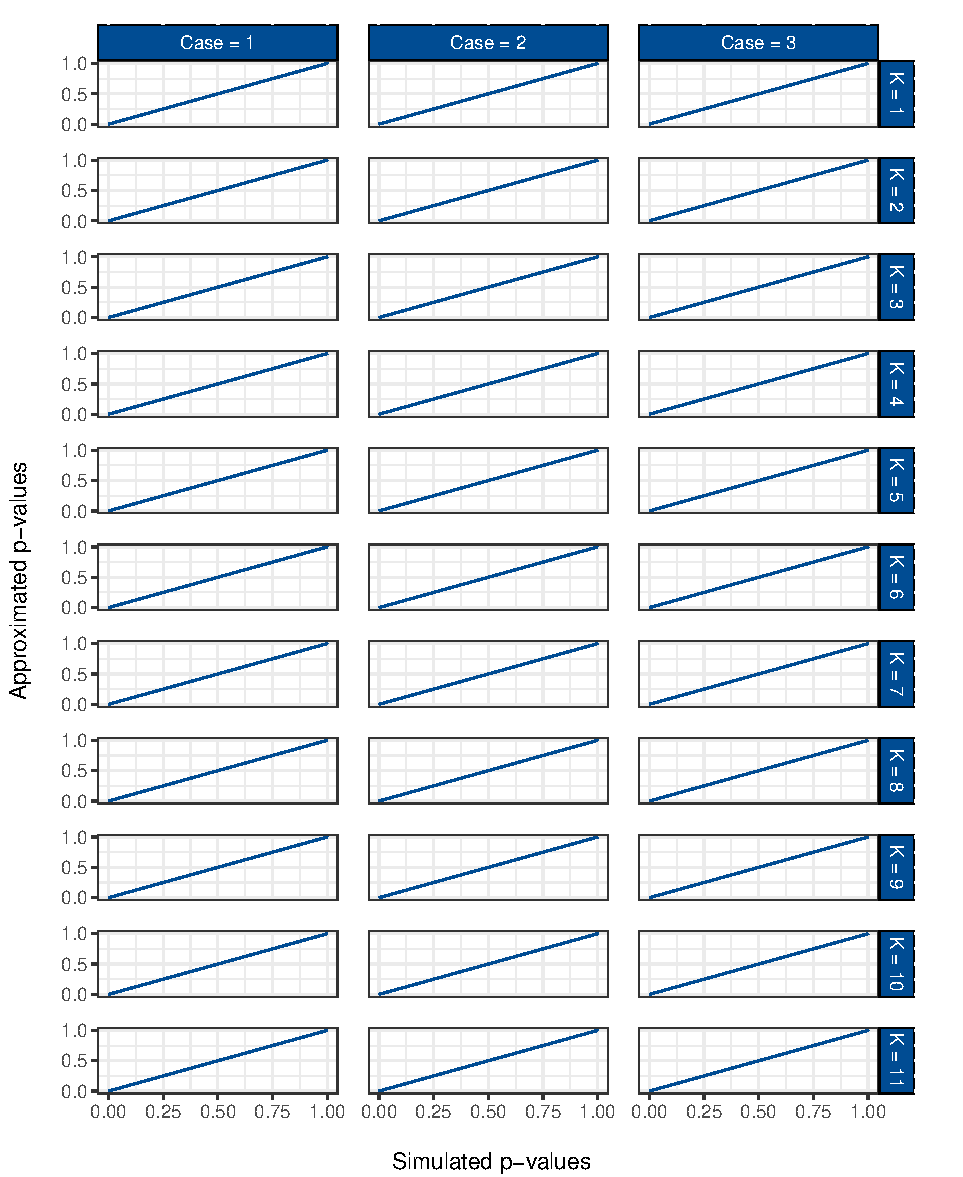
\includegraphics{p_approx_paper_files/figure-latex/approx_sim-all-1.pdf}
\caption{\label{fig:sim_approx_all} Simulated against approximated
\(p\)-values over the whole distribution for the first case and all
underlying tests included.}
\end{figure}

\begin{figure}
\centering
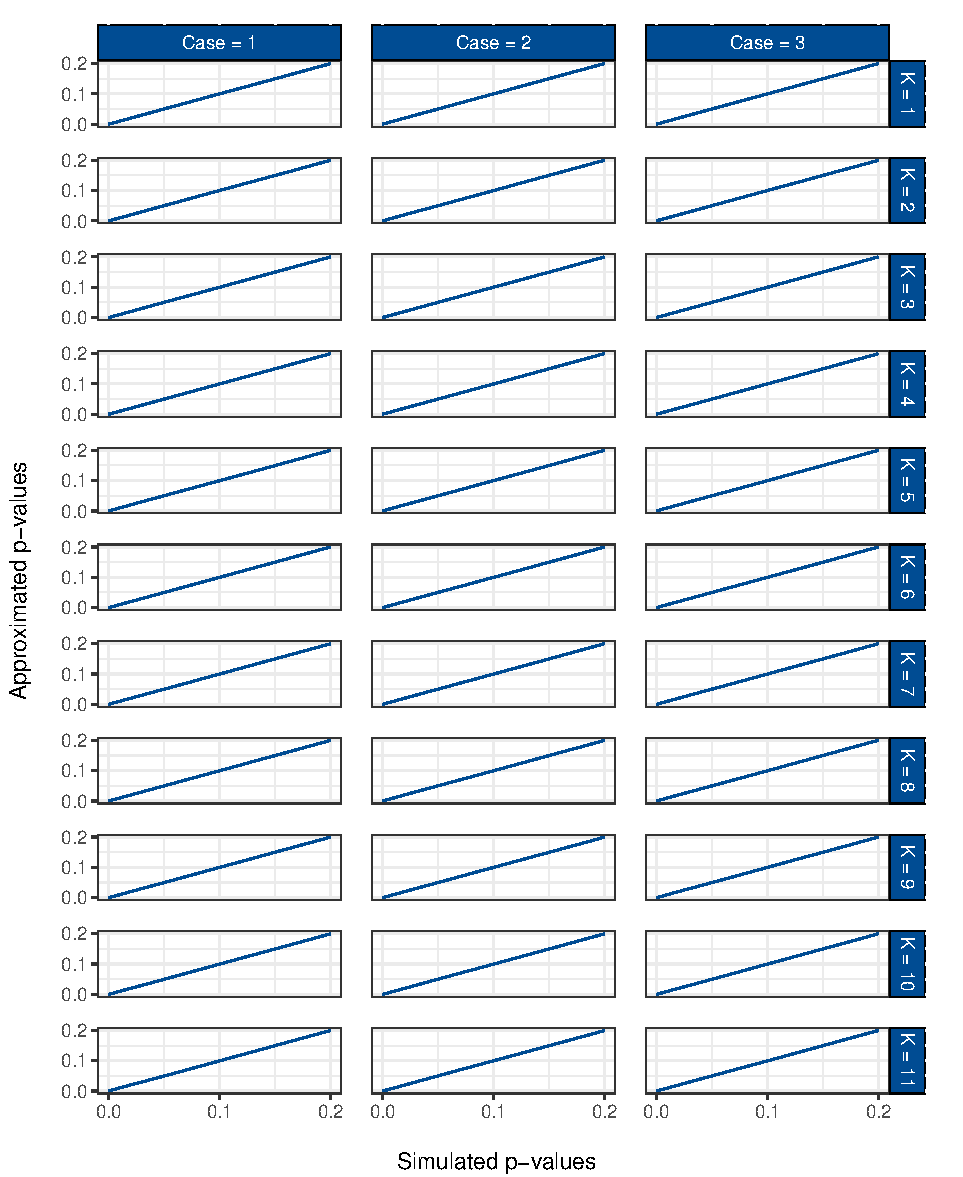
\includegraphics{p_approx_paper_files/figure-latex/approx_sim-all_0.2-1.pdf}
\caption{\label{fig:sim_approx_all_0.2} Simulated vs.~approximated
\(p\)-values for the lower tail of the distribution for the first case
and all underlying test included.}
\end{figure}

\begin{figure}
\centering
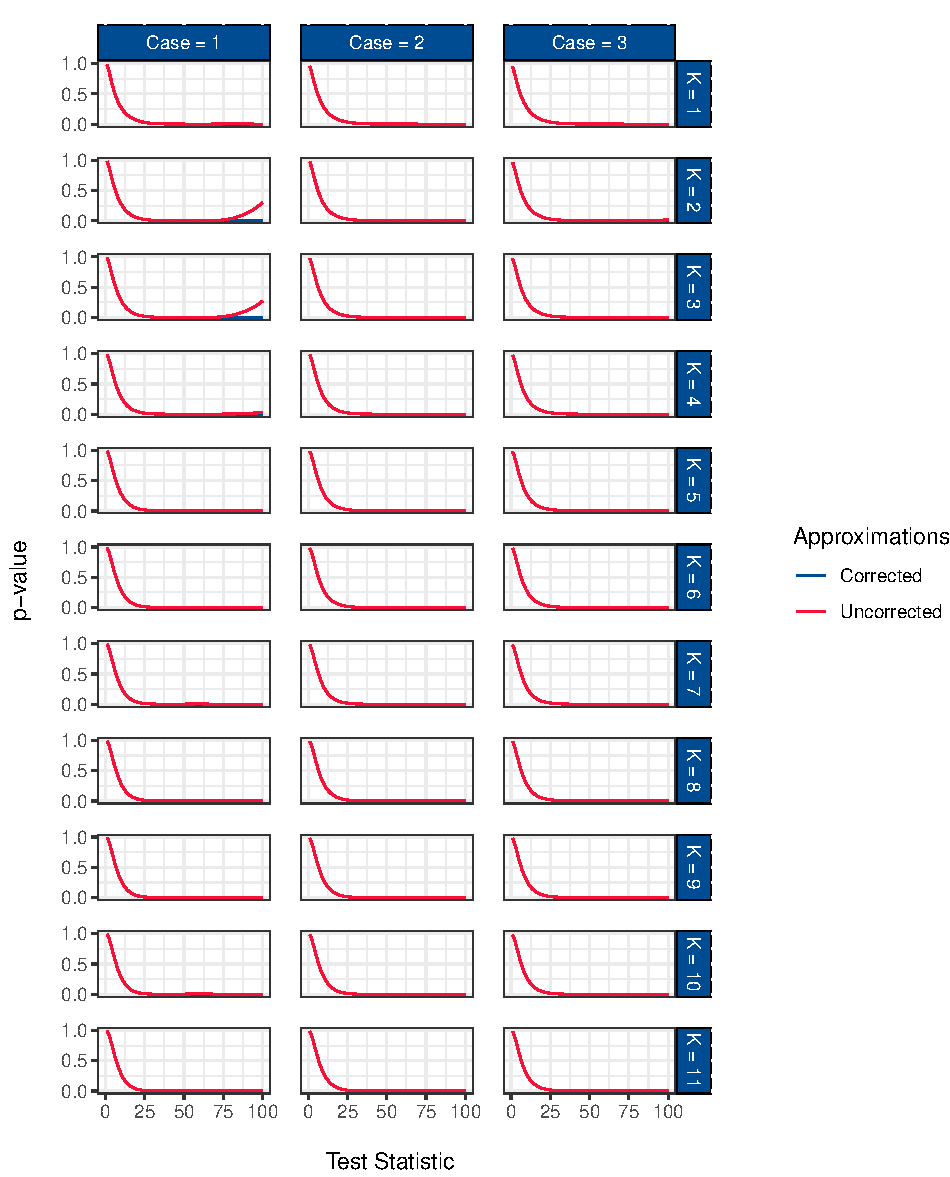
\includegraphics{p_approx_paper_files/figure-latex/p_stat_all-1.pdf}
\caption{\label{fig:fig_3} Corrected and uncorrected \(p\)-value
predictions for case 1 and all underlying tests included.}
\end{figure}

\begin{figure}
\centering
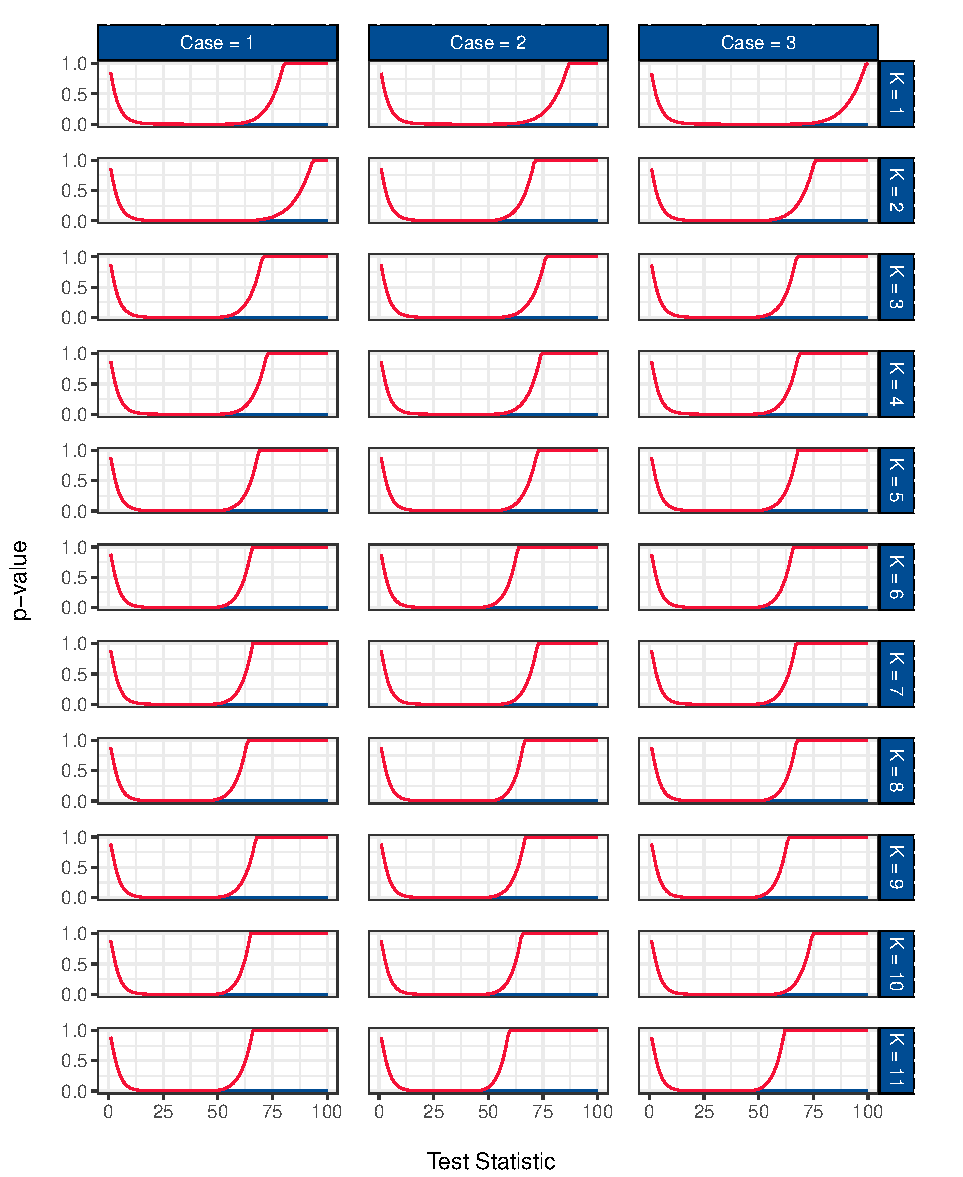
\includegraphics{p_approx_paper_files/figure-latex/p_stat_e_j-1.pdf}
\caption{\label{fig:fig_4} Corrected and uncorrected \(p\)-value
predictions for the first case using Johansen and Engle-Granger as
underlying tests.}
\end{figure}

\restoregeometry

\cleardoublepage
\newpage
\renewcommand*{\mkbibnamefamily}[1]{\textbf{#1}}
\renewcommand*{\mkbibnamegiven}[1]{\textbf{#1}}
\renewcommand*{\mkbibnameprefix}[1]{\textbf{#1}}
\renewcommand*{\mkbibnamesuffix}[1]{\textbf{#1}}


% \printbibliography[title=References]
%\pagenumbering{arabic}


\newpage
\textbf{Eidesstattliche Versicherung}

\bigskip

Ich versichere an Eides statt durch meine Unterschrift, dass ich die vorstehende Arbeit selbständig und ohne fremde Hilfe angefertigt und alle Stellen, die ich wörtlich oder annähernd wörtlich aus Veröffentlichungen entnommen habe, als solche kenntlich gemacht habe, mich auch keiner anderen als der angegebenen Literatur oder sonstiger Hilfsmittel bedient habe. Die Arbeit hat in dieser oder ähnlicher Form noch keiner anderen Prüfungsbehörde vorgelegen.

\vspace{1cm}
\rule{0pt}{2\baselineskip} %
\par\noindent\makebox[2.25in]{\indent Essen, den \hrulefill} \hfill\makebox[2.25in]{\hrulefill}%
\par\noindent\makebox[2.25in][l]{} \hfill\makebox[2.25in][c]{Jens Klenke
and Janine Langerbein}%


\end{document}
